\normalfalse \difficiletrue \tdifficilefalse
\correctiontrue

%\UPSTIidClasse{11} % 11 sup, 12 spé
%\newcommand{\UPSTIidClasse}{12}

\exer{Mouvement RR 3D  $\star\star$ \label{B2:13:08}}
\setcounter{numques}{0}
\UPSTIcompetence[2]{C2-05}
\UPSTIcompetence[2]{B2-13}
\index{Compétence C2-05}
\index{Compétence B2-13}
\index{Mécanisme à 2 rotations 3D}
\ifcorrection
\else
\textbf{Pas de corrigé pour cet exercice.}
\fi

\ifprof
\else
Soit le mécanisme suivant. On a $\vect{AB}=H\vect{j_1}+R\vect{i_1}$ et $\vect{BC}=L\vect{i_2}$. On a $H=\SI{20}{mm}$, $R=\SI{20}{mm}$, $L=\SI{10}{mm}$. 
\begin{center}
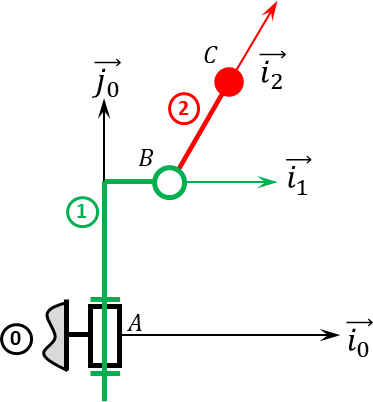
\includegraphics[width=\linewidth]{08_RR3D_01}
\end{center}
\fi

\question{Donner l'ensemble des positions accessibles par le point $C$.}
\ifprof
Le point $C$ peut décrire un tore de grand rayon $R$ et de petit rayon $L$ (surface torique uniquement, pas l'intérieur du tore). 
\else
\fi

\question{Donner l'équation de mouvement du point $C$ dans le mouvement de \textbf{2} par rapport à \textbf{0}.}
\ifprof ~\\
On  a  $\vect{AC}=H\vect{j_1}+R\vect{i_1}+L\vect{i_2}$ $=H\vj{0}+R\cos\theta\vi{0}-R\sin\theta\vk{0}+L\cos\varphi\vi{1}+L\sin\varphi\vj{1}$ 
$=H\vj{0}+R\cos\theta\vi{0}-R\sin\theta\vk{0}+L\cos\varphi\left(\cos\theta\vi{0}-\sin\theta\vk{0} \right)+L\sin\varphi\vj{0}$ .

On a donc :
$\left\{
\begin{array}{l}
x_C(t)=R\cos\theta+L\cos\varphi\cos\theta \\
y_C(t)= H+L\sin\varphi\\
z_C(t)=  -R\sin\theta-L\cos\varphi\sin\theta\\
\end{array}
\right.
$ dans le repère $\repere{A}{i_0}{j_0}{k_0}$.
\else
\fi

\ifprof
\else
\footnotesize
\begin{center}
\begin{tabular}{|p{.9\linewidth}|}
\hline
Indications
\begin{enumerate}
\item Tore.
\item $x_C(t)=R\cos\theta+L\cos\varphi\cos\theta$, $y_C(t)= H+L\sin\varphi$, $z_C(t)=  -R\sin\theta-L\cos\varphi\sin\theta$.
\end{enumerate} \\ \hline
\end{tabular}
\end{center}
\normalsize
\begin{flushright}
\footnotesize{Corrigé  voir \ref{B2:13:08}.}
\end{flushright}%
\fi